%%%%%%%%%%%%%%%%%%%%%%%%%%%%%%%%%%%%%%%%%%%%%%%%%%%%%%%%%%%%%%%%%%%%%%%%
%
% PREAMBOLO PER IL FILE ms.tex
%
%%%%%%%%%%%%%%%%%%%%%%%%%%%%%%%%%%%%%%%%%%%%%%%%%%%%%%%%%%%%%%%%%%%%%%%%

\begingroup
\thispagestyle{empty}
\AddToShipoutPicture*{\put(6,5){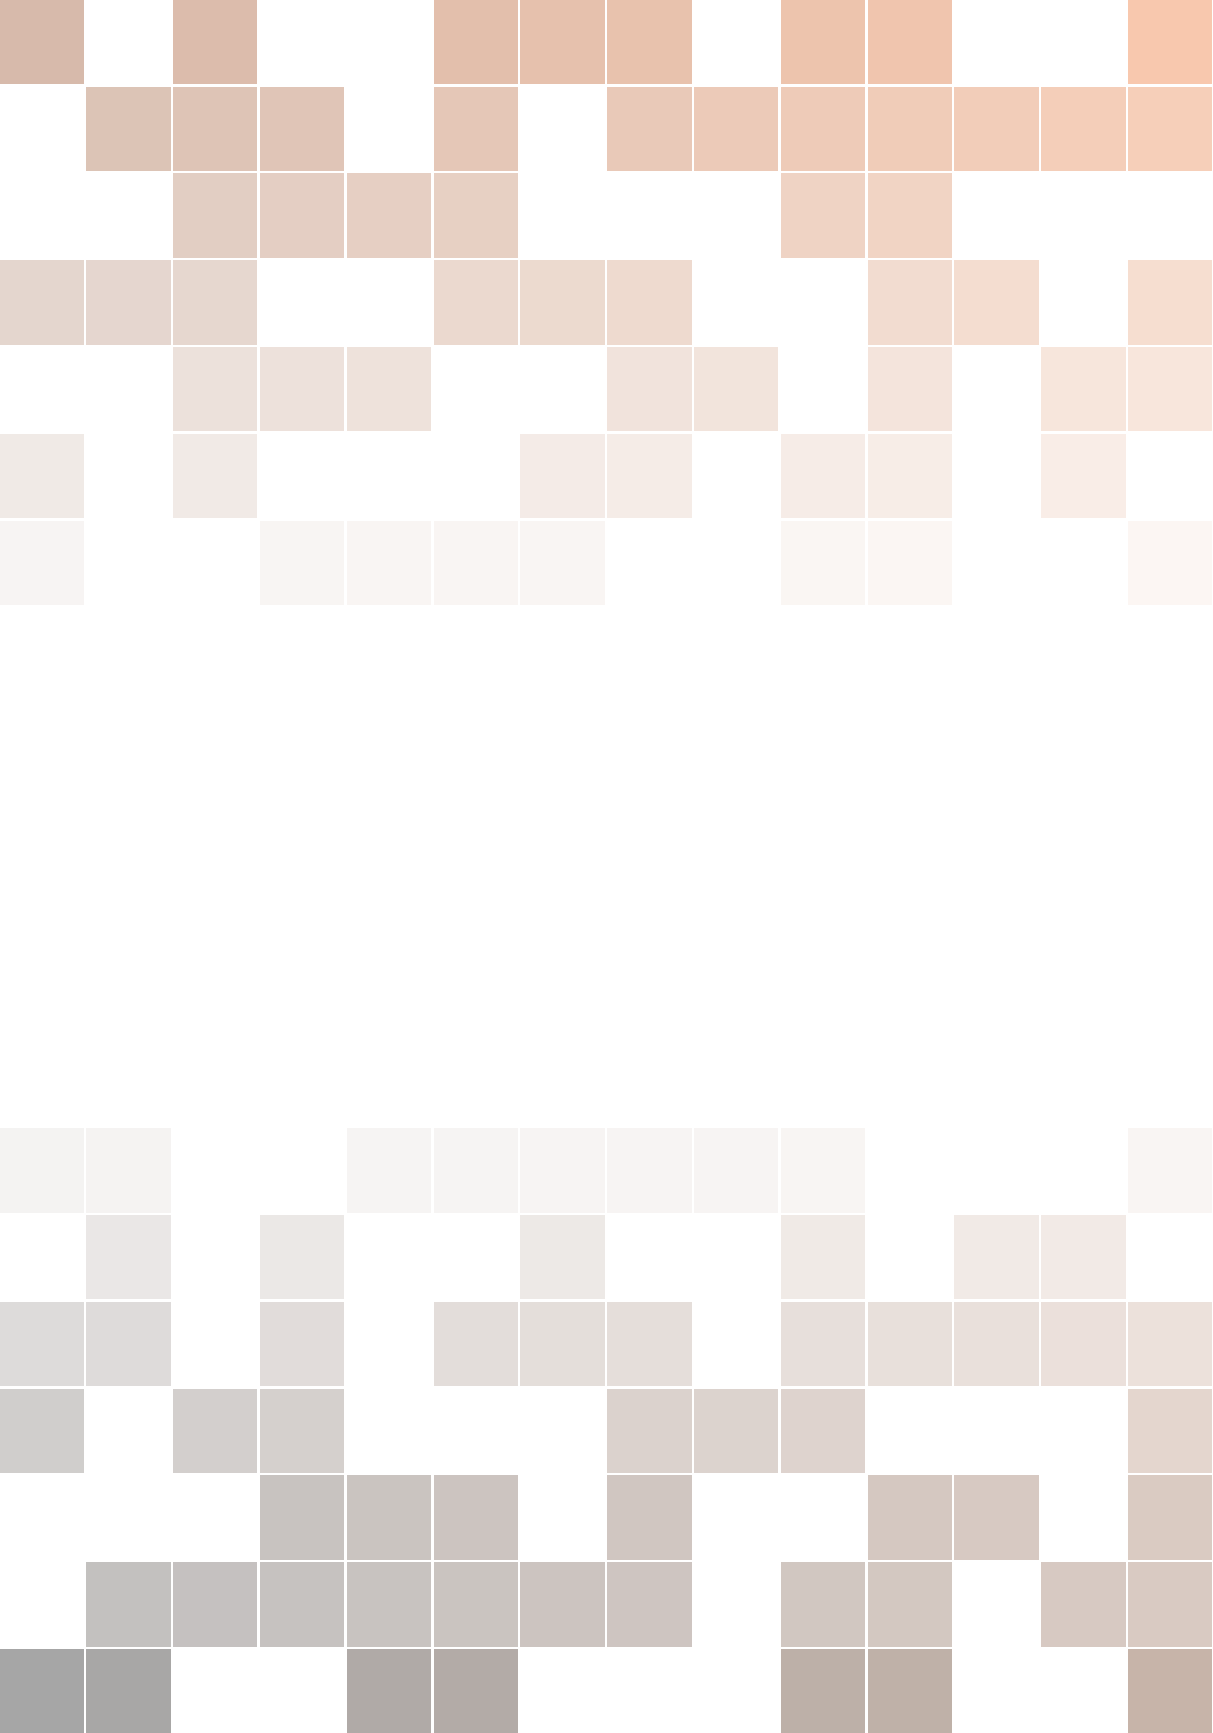
\includegraphics[scale=1]{background.pdf}}} % Image background
{\flushright
  \vspace*{6cm}
  \par\normalfont\fontsize{35}{35}\sffamily\selectfont
  Introduzione alla \\
  \vspace*{16pt}
  Meccanica Statistica\par % Book title
  \vspace*{2cm}
  {\huge Marco Guagnelli}\par % Author name
}
\endgroup

%----------------------------------------------------------------------------------------
%	COPYRIGHT PAGE
%----------------------------------------------------------------------------------------

\newpage
~\vfill
\thispagestyle{empty}

\noindent Copyright \copyright\ 2014--2017 Marco Guagnelli\\ % Copyright notice

\noindent www.pv.infn.it/\textasciitilde guagnelli/ms\\ % URL

\noindent These notes have been composed using the {\em memoir} package\\

\noindent Licensed under the Creative Commons Attribution-NonCommercial 3.0 Unported License (the ``License''). You may not use this file except in compliance with the License. You may obtain a copy of the License at \url{http://creativecommons.org/licenses/by-nc/3.0}. Unless required by applicable law or agreed to in writing, software distributed under the License is distributed on an \textsc{``AS IS'' BASIS, WITHOUT WARRANTIES OR CONDITIONS OF ANY KIND}, either express or implied. See the License for the specific language governing permissions and limitations under the License.\\ % License information

\noindent \textit{Versione 2.2, Aprile 2017} % Printing/edition date
\cleardoublepage

%----------------------------------------------------------------------------------------
%	TABLE OF CONTENTS
%----------------------------------------------------------------------------------------

\pagestyle{empty} % No headers
\tableofcontents % Print the table of contents itself
\cleardoublepage % Forces the first chapter to start on an odd page so it's on the right
\pagestyle{ruled} % Print headers again

%----------------------------------------------------------------------------------------

%%%%%%%%%%%%%%%%%%%%%%%%%%%%%%%%%%%%%%%%%%%%%%%%%%%%%%%%%%%%%%%%%%%%%%%%
\chapter*{Prefazione}
%%%%%%%%%%%%%%%%%%%%%%%%%%%%%%%%%%%%%%%%%%%%%%%%%%%%%%%%%%%%%%%%%%%%%%%%

\begin{minipage}{0.35\textwidth}\end{minipage}\hfill
\begin{minipage}{0.65\textwidth}
\flushright{\em
Un po' di saggezza è possibile, certo;\\
ma in tutte le cose\\
io ho trovato questa certezza beata:\\
che esse, sui piedi del caso,\\
preferiscono --- {\em danzare}.}
\vskip 0.25cm
\textsc{F. Nietzsche, ``Così parlò Zarathustra''}
\end{minipage}
\vskip 1.0cm

Queste dispense nascono dal corso di {\em Meccanica Statistica} che tengo dal 2010 presso il Dipartimento di Fisica dell'Università di Pavia. In prima istanza nascono dal tentativo, fatto a mio stesso beneficio, di mettere ordine nel caos di appunti manoscritti, su fogli spesso volanti, posti in anfratti altamente casuali, ed erraticamente vaganti col tempo, nel mio ufficio. Ogni anno dunque, nell'imminenza del corso, si ripropone la questione: {\em Dove diavolo saranno gli appunti per il metodo di Darwin--Fowler?} (sostituire a Darwin--Fowler un argomento a piacere e sommare su tutti i possibili argomenti del corso per ottenere il livello totale di frustrazione). Ho pensato che avrei speso meno tempo a cristallizzare in qualche forma digitale gli appunti stessi, per quindi ritrovarli velocemente da qualche parte sull'{\em hard disk} del mio {\em laptop}, che a cercarli ogni volta, nel disperato tentativo di diminuire l'entropia di cui riesco a circondarmi con enorme facilità. Spero comunque che questo piccolo sforzo sia utile anche agli studenti.

Il corso ha un carattere introduttivo alla materia e si rivolge a studenti del terzo anno della {\em Triennale} e/o del primo anno della {\em Specialistica}, o {\em Magistrale}. Gli argomenti sono quelli che ci si può facilmente aspettare: statistica classica, e quindi teoria degli \ensembles\ --- microcanonico, canonico, grancanonico; statistica quantistica, teoria dei gas ideali quantistici, termodinamica del corpo nero, calore specifico dei solidi, gas degenere di Fermi. Un capitolo è speso per la descrizione del modello di Ising e la sua soluzione in approssimazione di campo medio. Il corso presuppone la conoscenza, almeno a livello di corso di laurea in Fisica {\em Triennale}, della Termodinamica e della Meccanica Quantistica, oltre agli ovvi strumenti matematici necessari per qualsiasi corso di Fisica Teorica a questo livello.

Le dispense sono sostanzialmente una traduzione ragionata dei primi capitoli del Pathria, con alcune eccezioni. In ogni caso, più che plagiare brutalmente, ho cercato di dipanare la matassa del testo là dove mi sembrava più ingarbugliata.

Il testo è corredato da numerosi esercizi, che {\em fanno parte integrante del corso}. Le soluzioni degli esercizi si trovano in un altro volume. La maggior parte degli esercizi sono risolti durante le lezioni; consiglio vivamente agli studenti di provare a risolvere gli esercizi che non sono stati svolti a lezione {\em prima} di consultare il volume delle soluzioni.

Un lavoro del genere non può essere esente da {\em lapsi calami}, refusi e veri e propri errori; ringrazio tutti gli studenti che me li hanno già segnalati e ringrazio in anticipo chiunque avrà la bonta di segnalarmeli. Ringrazio in particolare la dott.ssa Barbara De Palma.
 
L'eventuale lettore dovrebbe avere la pazienza di considerare queste note come un {\em work in progress}, e tenere a mente il noto aforisma di Benjamin Disraeli: {\em The best way to become acquainted with a subject is to write a book about it}.

\vskip 1cm
\noindent
Pavia, Aprile 2017 \hfill Marco Guagnelli


